\documentclass[11pt,a4paper]{article}
\usepackage[margin=2.5cm]{geometry}
\usepackage{enumitem}
\usepackage{titlesec}
\usepackage{hyperref}
\usepackage{xcolor}
\usepackage{booktabs}
\usepackage{parskip}
\usepackage{graphicx}
\usepackage{amsmath}
\usepackage{amssymb}
\usepackage{float}

\definecolor{accent}{RGB}{30,70,120}
\definecolor{green}{RGB}{40,120,40}
\definecolor{red}{RGB}{180,40,40}

\titleformat{\section}{\large\bfseries\color{accent}}{\thesection.\ }{0.4em}{}[\titlerule]
\titleformat{\subsection}{\normalsize\bfseries\color{accent}}{\thesubsection\ }{0.4em}{}

\hypersetup{colorlinks=true, linkcolor=accent, urlcolor=accent}

\newcommand{\vhat}{\hat{v}}

\begin{document}

\begin{center}
{\LARGE\bfseries\color{accent} What the Bookmaker Pool Actually Computes}\\[0.5em]
{\large A Taylor decomposition of the momentum ratio, and a parameter-free correction}\\[1em]
{\small Robin Langer \quad|\quad September 2026}
\end{center}

\vspace{0.5em}

\begin{quote}
\small\itshape
The momentum signal in \texttt{momentum\_single.py} is shown to be exactly a ratio of two
products, whose logarithm expands into a volume--return covariance plus a second-order
curvature term. On the four equities tested the curvature term is comparable to or larger
than the covariance term in magnitude, and is structurally negative. Deleting it --- which
introduces no new free parameters --- flips the sign of the signal's edge on NVDA from
$-3.6$pp to $+4.6$pp and raises its correlation with forward returns on PLTR from $+0.34$
to $+0.46$. DE resists the correction and remains inverted.
\end{quote}

\section{The recursion collapses}

The implementation accumulates a ``pool'' over a window of $L$ daily returns $r_j$ with
volumes normalised by their window mean, $\vhat_j = v_j / \bar{v}$:

\begin{verbatim}
    pool = float(window_close[0]); mp = pool
    for j in range(len(net_flows)):
        pool += net_flows[j] * mp
        mp = pool
\end{verbatim}

Because \texttt{mp} is reassigned to \texttt{pool} on every iteration, the two variables are
never distinct. Writing $f_j = \vhat_j r_j$ for the net flow, the loop is simply
$\mathrm{mp}_{j+1} = \mathrm{mp}_j (1 + f_j)$, so

\[
\text{MomentumPrice} \;=\; P_0 \prod_{j=1}^{L} \bigl(1 + \vhat_j r_j\bigr).
\]

The denominator of the ratio is the realised final price, and since the $r_j$ are the actual
window returns, $P_T = P_0 \prod_j (1 + r_j)$ identically. The initial price cancels:

\begin{equation}
\boxed{\;\;
\text{MomentumRatio} \;=\; \frac{\prod_{j}\bigl(1 + \vhat_j r_j\bigr)}{\prod_{j}\bigl(1 + r_j\bigr)}
\;\;}
\label{eq:exact}
\end{equation}

This is an identity, not an approximation. Evaluated against the loop on NVDA over
2023--2026 ($L=180$, 750 windows), the maximum absolute discrepancy is
$5.6 \times 10^{-15}$ --- floating-point noise.

There is no bookmaker, no pool, and no betting dynamics. Equation~\eqref{eq:exact} compares
the path the asset \emph{did} take against a counterfactual path in which each day's return
was scaled by that day's relative volume.

\section{The expansion}

Take logarithms and expand each factor to second order in $r$:

\begin{align}
\log \text{MomentumRatio}
&= \sum_j \Bigl[ \log(1 + \vhat_j r_j) - \log(1 + r_j) \Bigr] \nonumber \\[0.3em]
&\approx \underbrace{\sum_j (\vhat_j - 1)\, r_j}_{\textstyle S \;=\; L \cdot \mathrm{Cov}(\vhat, r)}
\;\;-\;\; \underbrace{\tfrac{1}{2}\sum_j (\vhat_j^2 - 1)\, r_j^2}_{\textstyle D \;\text{(curvature drag)}}
\;+\; O(r^3).
\label{eq:expand}
\end{align}

The first-order term is exactly $L$ times the sample covariance of normalised volume with
return, because $\overline{\vhat} = 1$ by construction and hence
$\sum_j (\vhat_j - 1) r_j = L\bigl(\overline{\vhat r} - \overline{\vhat}\,\overline{r}\bigr)$.

\subsection*{What each term means}

\textbf{$S$, the signal.} The covariance of volume with return is a real and well-studied
quantity: it is positive when up-days trade heavier than down-days. Thresholding on it is a
defensible strategy, and it is what the model was presumably intended to measure.

\textbf{$D$, the drag.} This term has no directional content whatsoever. It depends on $r_j^2$,
so it cannot distinguish a rise from a fall. Worse, it is structurally negative: by Jensen's
inequality $\overline{\vhat^2} \geq \overline{\vhat}^2 = 1$, so the weights $(\vhat_j^2 - 1)$ are
positive on average, and $D$ subtracts a quantity that scales with realised \emph{variance}
times volume dispersion.

The consequence is that the ratio is pushed below $1$ for any asset that is volatile and has
dispersed volume --- independently of direction. Since the strategy goes long when the ratio
exceeds $1$, it systematically refuses to hold exactly the high-volatility assets whose
returns are most worth holding.

\subsection*{Magnitudes}

Table~\ref{tab:mag} decomposes the mean log ratio over 2021--2026 at $L=180$.

\begin{table}[H]
\centering
\small
\begin{tabular}{lrrrrr}
\toprule
& \textbf{mean $\log$ ratio} & \textbf{signal $S$} & \textbf{drag $D$} & $|D|/|S|$ & \textbf{ann.\ vol} \\
\midrule
NVDA & $-0.032$ & $+0.103$ & $-0.143$ & $1.38$ & $52.1\%$ \\
AMD  & $+0.216$ & $+0.407$ & $-0.239$ & $0.59$ & $57.4\%$ \\
DE   & $-0.239$ & $-0.108$ & $-0.096$ & $0.89$ & $29.8\%$ \\
PLTR & $+0.018$ & $+0.736$ & $-0.856$ & $1.16$ & $67.0\%$ \\
\bottomrule
\end{tabular}
\caption{The drag is of the same order as the signal, and larger on two of four names.
On NVDA and PLTR it is large enough to reverse the sign of the mean log ratio.}
\label{tab:mag}
\end{table}

NVDA is the clearest case. Its signal term is \emph{positive} ($+0.103$): volume genuinely
did concentrate on up-days. But the drag ($-0.143$) is larger, so the ratio averages below
$1$ and the strategy sits in cash. This is the mechanism behind the $-1329$pp alpha recorded
for NVDA in the backtest --- the model held for only $43.5\%$ of days across a period in
which buy-and-hold returned $+1529\%$.

\begin{figure}[H]
\centering
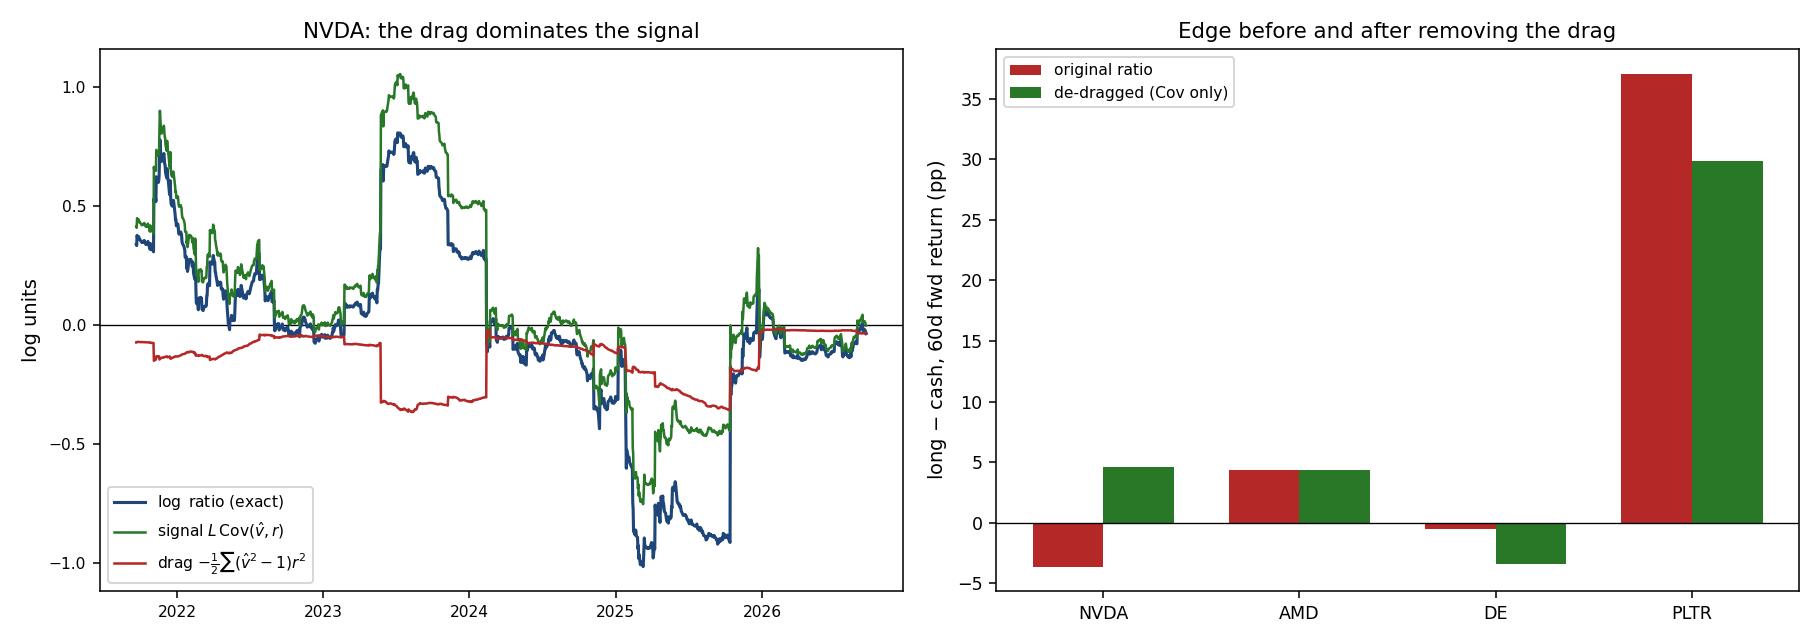
\includegraphics[width=\textwidth]{taylor_decomposition.png}
\caption{Left: the decomposition over time for NVDA. The blue curve (the exact log ratio) tracks
the red drag more closely than the green signal. Right: the spread in 60-day forward return
between long and cash states, before and after removing the drag.}
\end{figure}

\section{The correction and its test}

The correction is to threshold on $S > 0$ rather than on the full ratio exceeding $1$ ---
that is, to delete $D$ from equation~\eqref{eq:expand}. This introduces \textbf{no new free
parameters}: no threshold is tuned, no lookback swept, no weighting fitted. A term identified
as directionless on analytic grounds is simply removed.

\begin{table}[H]
\centering
\small
\begin{tabular}{lrrrrrr}
\toprule
& \multicolumn{2}{c}{\textbf{original ratio}} & \multicolumn{2}{c}{\textbf{de-dragged ($S>0$)}}
& \multicolumn{2}{c}{\textbf{corr with fwd60}} \\
\cmidrule(lr){2-3}\cmidrule(lr){4-5}\cmidrule(lr){6-7}
& spread (pp) & sign & spread (pp) & sign & ratio & $S$ \\
\midrule
NVDA & $-3.6$  & \textcolor{red}{$\times$} & $+4.6$  & \textcolor{green}{$\checkmark$} & $-0.068$ & $-0.066$ \\
AMD  & $+4.4$  & \textcolor{green}{$\checkmark$} & $+4.3$  & \textcolor{green}{$\checkmark$} & $+0.095$ & $+0.205$ \\
DE   & $-0.6$  & \textcolor{red}{$\times$} & $-3.4$  & \textcolor{red}{$\times$} & $-0.132$ & $-0.161$ \\
PLTR & $+37.0$ & \textcolor{green}{$\checkmark$} & $+29.9$ & \textcolor{green}{$\checkmark$} & $+0.339$ & $+0.457$ \\
\bottomrule
\end{tabular}
\caption{Spread is the mean 60-day forward return when long minus when in cash. Removing the
drag flips NVDA's sign and materially improves the correlation on AMD ($+0.095 \to +0.205$)
and PLTR ($+0.339 \to +0.457$).}
\label{tab:fix}
\end{table}

Three of four names now point the right way, and the two names where the correlation improves
most are the two with the largest drag-to-signal ratio --- which is the direction the theory
predicts.

\section{The DE anomaly}

DE does not merely fail to improve; the correction makes it worse ($-0.6$pp to $-3.4$pp,
correlation $-0.132$ to $-0.161$). Removing a directionless term made a wrong signal
\emph{more} wrong, which means DE's covariance term genuinely carries the opposite sign: on
Deere, heavy volume on up-days preceded \emph{lower} forward returns over this window.

This is now the interesting residual rather than noise. A plausible reading is that for a
low-volatility industrial, volume spikes mark institutional rebalancing and index flows
rather than directional conviction, so $\mathrm{Cov}(\vhat, r)$ measures supply being met
rather than demand arriving. That is a hypothesis with a clean test, stated below.

\section{Limitations}

\begin{enumerate}[leftmargin=1.4em]
\item \textbf{Four names, one window.} Everything here runs from January 2021 to September
2026 --- a period containing the largest semiconductor repricing in decades. Three
observations pointing the right way is suggestive, not significant.
\item \textbf{Overlapping windows.} The forward-return buckets use 60-day horizons sampled
daily, so of $\sim$1300 rows only about $\sim$21 are independent. The correlations are
computed on heavily autocorrelated data and their standard errors are much wider than the
sample size suggests.
\item \textbf{In-sample.} The correction was derived by inspecting the same assets it is
tested on. Its parameter-free character is the reason to take it seriously, but it is not a
substitute for out-of-sample validation.
\item \textbf{No costs.} All figures are gross of commission, spread, and slippage.
\item \textbf{Signal only.} This document analyses the signal's relationship to forward
returns. It does not constitute a backtest of a corrected strategy, and says nothing about
position sizing or drawdown.
\end{enumerate}

\section{Next tests}

\begin{enumerate}[leftmargin=1.4em]
\item \textbf{Out-of-sample on the existing suite.} The repository already contains computed
timing files for BTC, ETH, SOL, six FX futures, and five commodities. Re-running those with
the de-dragged signal tests an equity-derived correction on fifteen assets it was not derived
from --- the cheapest genuine out-of-sample check available.
\item \textbf{Does the sign of $\mathrm{Cov}(\vhat,r)$ sort by volatility or sector?}
Compute the correlation across 50--100 names and regress it on realised volatility, market
capitalisation, and sector. If DE's inversion is systematic among low-volatility industrials,
the result is a rule for \emph{when} the signal applies, which is worth more than the signal.
\item \textbf{Lookback sweep, as a prediction rather than a fit.} The drag accumulates as
$L\sigma^2$ while the signal accumulates as $L\,\mathrm{Cov}$. Removing $D$ should therefore
shift the optimal $L$ in a predictable direction. Sweeping $L$ before and after the
correction tests that prediction; sweeping it only afterwards would merely be fitting.
\end{enumerate}

\vspace{1em}
\hrule
\vspace{0.5em}
{\footnotesize Reproduced from \texttt{momentum\_single.py} at $L = 180$, daily closes and
volumes from \texttt{yfinance}, 2021-01-01 to 2026-09-20. Figure:
\texttt{taylor\_decomposition.png}.}

\end{document}
